
\de{ĐỀ THI GIỮA HỌC KỲ II NĂM HỌC 2022-2023}{THPT Lê Trọng Tấn}

\begin{bt}%[Dự án đề kiểm tra GHKII NH22-23- Thầy Hoá]%[0T7B2-1]
Giải các bất phương trình sau 
\begin{listEX}[2]
\item $2x^2-5x+2<0$;
\item $2(x-1)^2 \geq 3x^2+6x+27$.
\end{listEX}
\loigiai{\begin{enumerate}
\item Xét $2x^2-5x+2=0\Leftrightarrow \hoac{&x=2\\&x=\dfrac{1}{2}.}$\\
Bảng xét dấu
\begin{center}
\begin{tikzpicture}
	\tkzTabInit[nocadre=false,lgt=3.5,espcl=3,deltacl=0.5]{$x$/1 ,$2x^2-5x+2$/1}
	{$-\infty$ , $\tfrac{1}{2}$ , $2$ , $+\infty$}
	\tkzTabLine{ , + , 0 , - , 0 , + ,  }
\end{tikzpicture}
\end{center}
Dựa vào bảng xét dấu, tập nghiệm của bất phương trình là $S=\left(\dfrac{1}{2};2\right)$.
\item Ta có
\begin{eqnarray*}
	2(x-1)^2 \geq 3x^2+6x+27&\Leftrightarrow&2(x^2-2x+1) \ge 3x^2 +6x+27\\
	&\Leftrightarrow&x^2+10x+25\le 0\\
	&\Leftrightarrow&(x+5)^2\le 0\\
	&\Leftrightarrow&x=-5.
\end{eqnarray*}
Tập nghiệm của bất phương trình là $S=\{-5\}$.
\end{enumerate}
}
\end{bt} 

\begin{bt}%[Dự án đề kiểm tra GHKII NH22-23- Thầy Hoá]%[0T7B2-1]
Tìm tất cả các giá trị thực của tham số $m$ để $f(x)=x^2-(m-2)x+8m+1 \geq 0$, $\forall x \in \mathbb{R}$.
\loigiai{
Bất phương trình đúng với mọi $x \in \mathbb{R}$ khi và chỉ khi
\[\heva{
	& a=1 >0~(\text{luôn đúng}) \\
	& \Delta =(m-2)^2-4 \cdot (8m+1) \leq 0 
} \Leftrightarrow m^2-36m \leq 0 \Leftrightarrow m \in [0;36]. \]
Vậy với $m \in [0;36]$ thỏa mãn yêu cầu bài toán.
}
\end{bt}

\begin{bt}%[Dự án đề kiểm tra GHKII NH22-23- Thầy Hoá]%[0T7B3-2]
Giải các phương trình sau
\begin{listEX}[2]
\item $\sqrt{x+2}=\sqrt{3x^2-x+1}$;
\item $\sqrt{x^2-4x+5}+2x=3$.
\end{listEX}
\loigiai{
\begin{listEX}[1]
	\item $\begin{aligned}[t]
		&\sqrt{x+2}=\sqrt{3x^2-x+1}\\
		\Rightarrow &x+2=3x^2-x+1\\
		\Leftrightarrow &3x^2-2x-1=0\\
		\Leftrightarrow &\hoac{&x=1\\&x=\dfrac{-1}{3}.}
	\end{aligned}$\\
	Thế $x=1$ và $x=\dfrac{-1}{3}$ vào phương trình đã cho, ta thấy đều thỏa mãn.\\
	Vậy tập nghiệm của   phương trình là $ S=\left \{-\dfrac{1}{3};1\right \} $.
	\item $\begin{aligned}[t]
		&\sqrt{x^2-4x+5}+2x=3\\
		\Leftrightarrow &\sqrt{x^2-4x+5}=3-2x\\
		\Rightarrow &x^2-4x+5=(3-2x)^2\\
		\Leftrightarrow &x^2-4x+5=9-12x+4x^2\\
		\Leftrightarrow &3x^2-8x+4=0\\
		\Leftrightarrow &\hoac{&x=2\\&x=\dfrac{2}{3}.}
	\end{aligned}$\\
Thế $x=2$ và $x=\dfrac{2}{3}$ vào phương trình ban đầu, ta thấy giá trị $x=\dfrac{2}{3}$ thỏa mãn.\\
Vậy tập nghiệm của   phương trình là $ S=\left \{\dfrac{2}{3} \right \} $.
\end{listEX}
}
\end{bt}

\begin{bt}%[Dự án đề kiểm tra GHKII NH22-23- Thầy Hoá]%[0T3K2-5]
\immini{
Xét hệ tọa độ $Oth$ trên mặt phẳng, trong đó trục $Ot$ biểu thị thời gian $t$ (tính bằng giây) và trục $Oh$ biểu thị độ cao so với mặt đất (tính bằng mét). Một quả bóng được đá lên từ độ cao $20$ (cm) so với mặt đất và chuyển động theo quỹ đạo là một cung parabol. Quả bóng đạt độ cao $8{,}5$ (m) so với mặt đất sau $1$ giây và đạt độ cao $6$ (m) so với mặt đất sau $2$ giây. Hỏi quả bóng ở độ cao trên $7$ (m) so với mặt đất trong khoảng thời gian bao nhiêu giây? (làm tròn kết quả đến hàng phần trăm)
}{
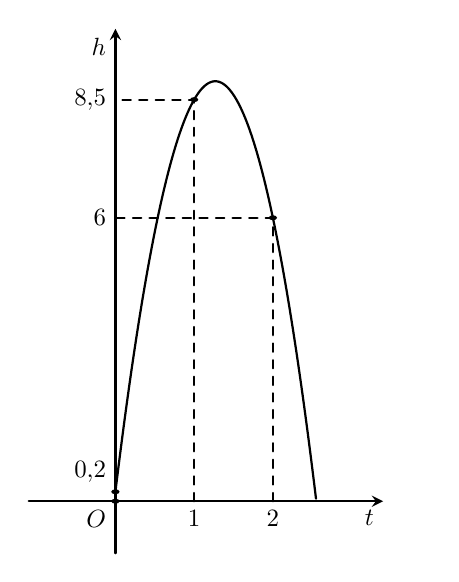
\begin{tikzpicture}[line join=round, line cap=round,>=stealth,thick,yscale=0.6]
\tikzset{every node/.style={scale=0.9}}
\draw[->] (-1.1,0)--(3.4,0) node[below left] {$t$};
\draw[->] (0,-1.1)--(0,10) node[below left] {$h$};
\draw (0,0) node [below left] {$O$};
\draw[dashed] (1,0) node[below]{$ 1 $}--(1,8.5)--(0,8.5)node[left]{$ 8{,}5 $};
\draw[dashed] (2,0) node[below]{$ 2 $}--(2,6)--(0,6)node[left]{$ 6 $};
\draw (0,0.2) node[above left]{$ 0{,}2 $};
\begin{scope}
	\clip (-1,-1) rectangle (4,10);
	\draw[samples=200,domain=0:2.55,smooth,variable=\x] plot (\x,{-27/5*(\x)^2+137/10*(\x)+0.2});
\end{scope}
\fill (0,0) circle (1.5pt);
\fill (2,6) circle (1.5pt);
\fill (1,8.5) circle (1.5pt);
\fill (0,0.2) circle (1.5pt);
\end{tikzpicture}}
\loigiai{Quỹ đạo của quả bóng là parabol $(P)\colon h(t)=at^2+bt+c$.
\begin{itemize}
	\item Lúc $t=0$ ta có $h=c=0{,}2$.
	\item Lúc $t=1$ ta có $h=a+b+0{,}2=8{,}5 \Leftrightarrow a+b=8{,}3$.
	\item Lúc $t=2$ ta có $h=4a+2a+0{,}2=6 \Leftrightarrow 4a+2b=5{,}8$.
\end{itemize}
Suy ra $a=-\dfrac{27}{5}$; $b=\dfrac{137}{10}$; $c=0{,}2$.\\
Với $h=7$ ta có $-\dfrac{27}{5}t^2+\dfrac{137}{10}t+0{,}2=7 \Leftrightarrow \hoac{& t\approx 0{,}68\\&t \approx 1{,}86.}$ \\
Do đó khoảng thời gian quả bóng trên $ 7 $ m so với mặt đất xấp xỉ
\[1{,}86-0{,}68=1{,}18\ (\text{giây}). \]
}
\end{bt}

\begin{bt}%[Dự án đề kiểm tra GHKII NH22-23- Thầy Hoá]%[0T9B2-2]
Cho tam giác $ABC$ có $A(-2;1)$, $B(1;2)$, $C(4;-1)$.
\begin{enumerate}
\item Tính độ dài các cạnh $AB$ và $BC$ của tam giác $ABC$.
\item Tìm tọa độ điểm $E$ là hình chiếu của $A$ lên trục hoành và tính khoảng cách từ $E$ đến $B$.
\item Viết phương trình tổng quát của đường thẳng $AC$ và phương trình tham số đường cao $AH$ của tam giác $ABC$.
\item Viết phương trình đường thẳng $\Delta$ song song với $(d):2x+y+2=0$ và cách $A$ một khoảng bằng $\dfrac{1}{\sqrt{5}}$.
\end{enumerate} 
\loigiai{
\begin{enumerate}
\item Ta có $\overrightarrow{AB}=(3;1) \Rightarrow AB=\sqrt{3^2+1^2}=\sqrt{10}$.\\
Và $\overrightarrow{BC}=(3;-3) \Rightarrow BC=\sqrt{3^2+(-3)^2}=3\sqrt{2}$.
\item Vì $E$ là hình chiếu của $A$ lên trục hoành nên $x_E=x_A=-2$ và $y_E=0$, suy ra $E(-2;0)$.\\
Ta có $\vec{EB}=(3;2)$, suy ra $EB=\sqrt{3^2+2^2}=\sqrt{13}$.
\item Véc-tơ chỉ phương $\vec{AC}=(6;-2)$, suy ra véc-tơ pháp tuyến $\vec{n}=(2;6)$.\\
Phương trình tổng quát của đường thẳng $AC$ đi qua $A(-2;1)$ có véc-tơ pháp tuyến $\vec{n}=(2;6)$ là
\[2(x+2)+6(y-1)=0\Leftrightarrow 2x+6y-2=0\Leftrightarrow x+3y-1=0. \]
Vậy $AC\colon x+3y-1=0$.\\
Đường cao $AH$ vuông góc với $BC$ nên nhận $\vec{BC}=(3;-3)$ làm véc-tơ pháp tuyến, suy ra véc-tơ chỉ phương $\vec{u}=(3;3)$. Chọn véc-tơ chỉ phương $\vec{u'}=(1;1)$.\\
Phương trình tham số của đường thẳng $AH$ đi qua $A(-2;1)$, có véc-tơ chỉ phương $\vec{u'}=(1;1)$ là
\[AH\colon\heva{&x=-2+t\\&y=1+t}~(t \in \mathbb{R}). \]
\item Vì $\Delta$ song song với $(d):2x+y+2=0$ nên $\Delta\colon  2x+y+c=0$ ($c \neq 2$).\\
Lại có $\mathrm{d}(A;\Delta)=\dfrac{1}{\sqrt{5}}\Leftrightarrow\dfrac{\left|2(-2)+1+c\right|}{\sqrt{2^2+1^2}}=\dfrac{1}{\sqrt{5}} \Leftrightarrow |c-3|=1 \Leftrightarrow \hoac{
	& c=4~(\text{nhận}) \\
	& c=2~(\text{loại}). \\
}$\\
Vậy $\Delta\colon 2x+y+4=0$.
\end{enumerate}
}
\end{bt}
